\subsection{Electrical Measurement Distributions from Experimental Literature}% Data of Neuroelectro 
%Origins}
As described elsewhere ephysiological measurement distributions were sourced from neuro-electro \cite{tripathy2014neuroelectro}. It is unwise to utilize data in almost every application without first visualizing it, and potentially cleaning it.\\
\\
In many instances the mean and standard deviation well describe the electrical measurements, that were fitted to models, occasionally they do not. A few different interesting cases are explored below.

\begin{comment}

\begin{figure}
\begin{center}
\centering
\begin{subfigure}{scale=0.5}
  \centering
   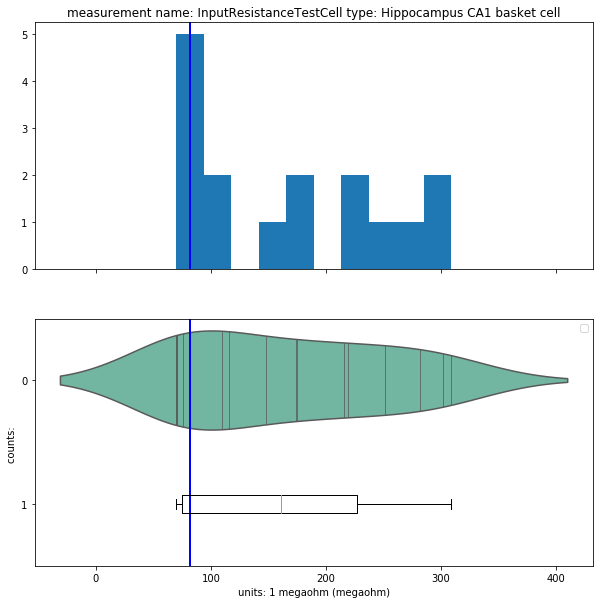
\includegraphics[scale=0.45]{notebooks_converted/needata_thesis_files/needata_thesis_5_5}
%\caption{Model parameterization of the brian2 simulator with the customization: interpolated spike height, forced to be above $0mV$}

  \label{fig:sub1}
\end{subfigure}%
\begin{subfigure}{scale=0.5}
  \centering
  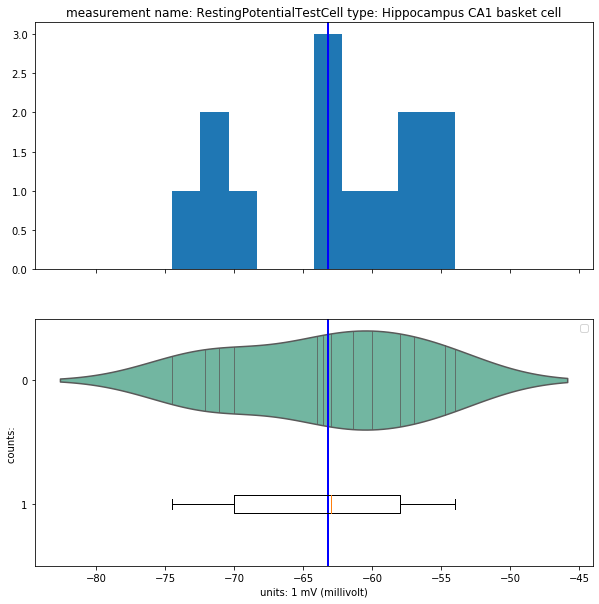
\includegraphics[scale=0.45]{notebooks_converted/needata_thesis_files/needata_thesis_5_6}
    
    %\caption{Default model parameterization of the custom written integrator}
  \label{fig:sub2}
\end{subfigure}

\begin{subfigure}{scale=0.5}
  \centering
      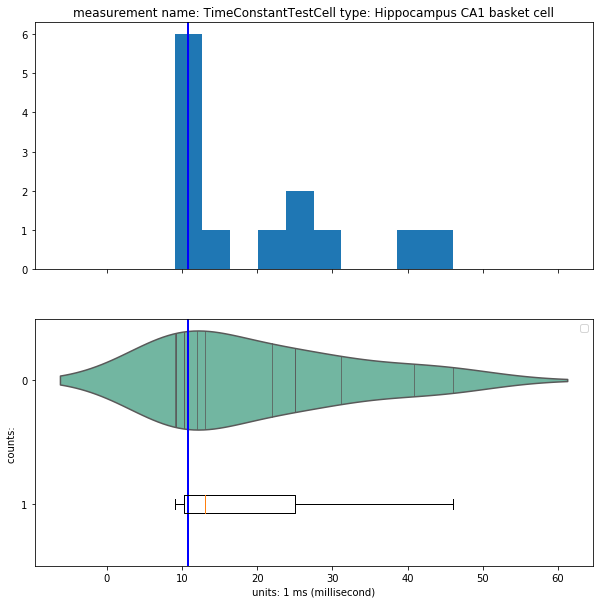
\includegraphics[scale=0.45]{notebooks_converted/needata_thesis_files/needata_thesis_5_7}
      %\caption{Default model parameterization of the custom written integrator}
  \label{fig:sub2}
\end{subfigure}

%\caption{Comparison between two Adxaptive Exponential Implementations}
\label{fig:test}
\end{center}
\end{figure}

\end{comment}

    
    %\begin{center}
    %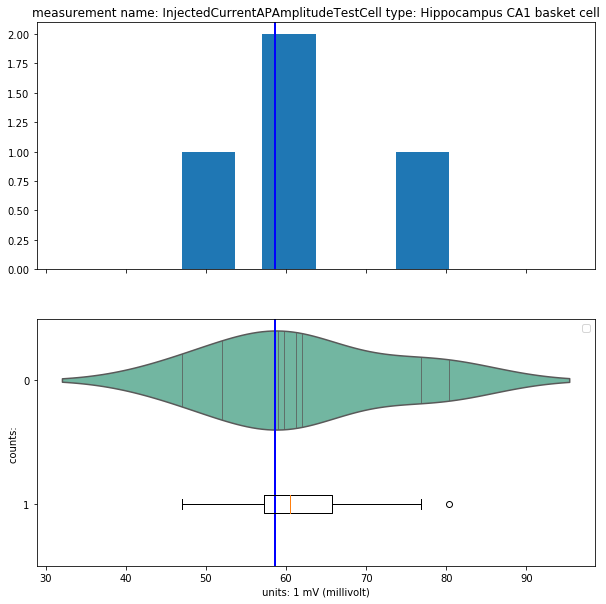
\includegraphics[width=0.7\linewidth]{notebooks_converted/needata_thesis_files/needata_thesis_5_8}
    %\end{center}
    %
    
\begin{figure} 
    \begin{center}

   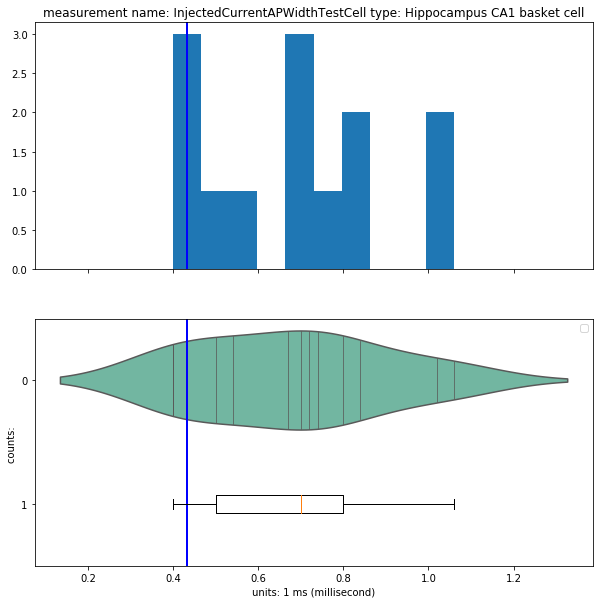
\includegraphics[scale=0.45]{notebooks_converted/needata_thesis_files/needata_thesis_5_9}
   \caption{The Action Potential Width of the Hippocampus CA1 basket cell possibly has either an underlying uniform distribution or a multimodal distribution. Since the samples are few, the true distribution is unknown. If the distribution is uniform the gaps in the distribution, that give the histogram a multimodal appearance, as the sample size is lower enough that such gaps may only represent missing samples.}
    \end{center}

\end{figure}
    { \hspace*{\fill} \\}

   \begin{figure}   
\begin{center}

   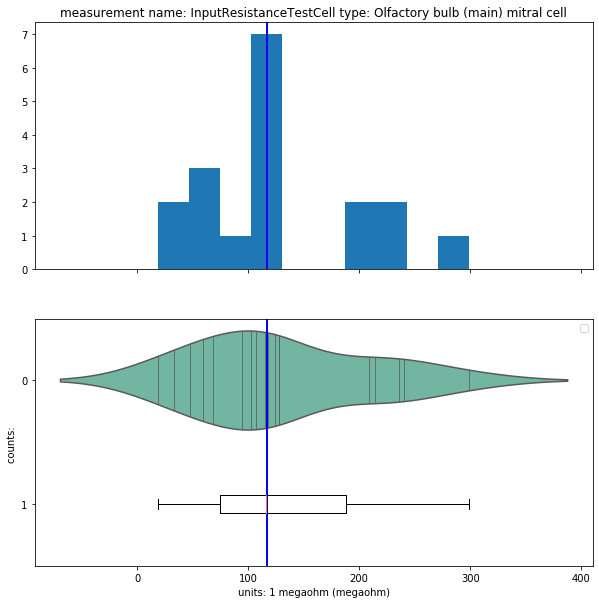
\includegraphics[scale=0.45]{notebooks_converted/needata_thesis_files/needata_thesis_5_21}
         \caption{Input resistance of the Olfactory Mitral cell showed some tendency towards underlying bi-modal distribution, however the second block of histogram bins, centered around $200-300pA$ only contains approximately $5$ samples}
\end{center}

   \end{figure}
   
\begin{figure}  
\begin{center}     

  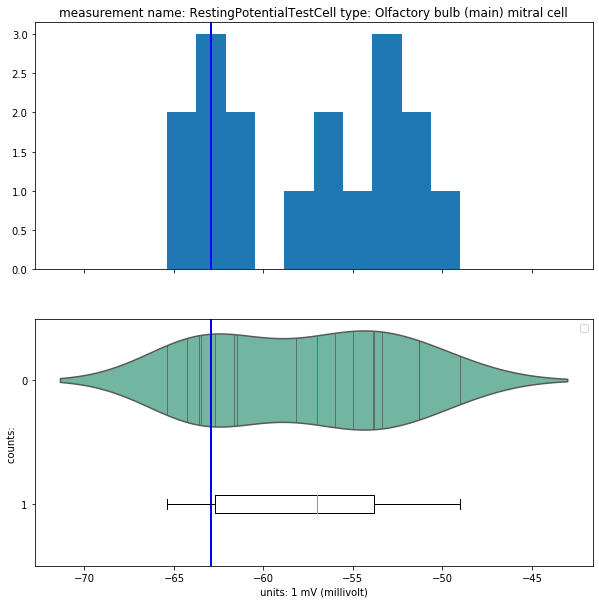
\includegraphics[scale=0.45]{notebooks_converted/needata_thesis_files/needata_thesis_5_22}
      \caption{Among different measurement sources of neuroelectro data, the resting membrane potential of the Olfactory Mitral cell, showed the greatest tendency of an underlying bi-modal distribution
      In the top panel of this plot we see a binned histogram of Resting membrane potential in the olfactory mitrall cell      
      }

\end{center}     
\end{figure}



\begin{figure}
  \centering
  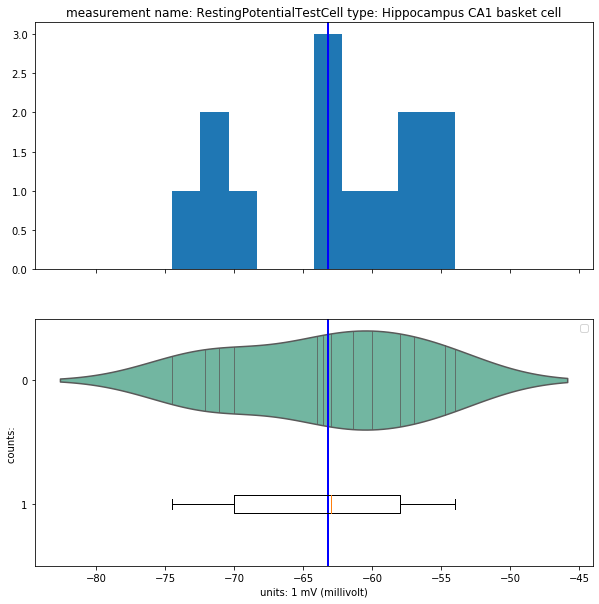
\includegraphics[scale=0.45]{notebooks_converted/needata_thesis_files/needata_thesis_5_6}
    
    %\caption{Default model parameterization of the custom written integrator}
  \label{fig:sub2}
\end{figure}

%    \begin{center}
%   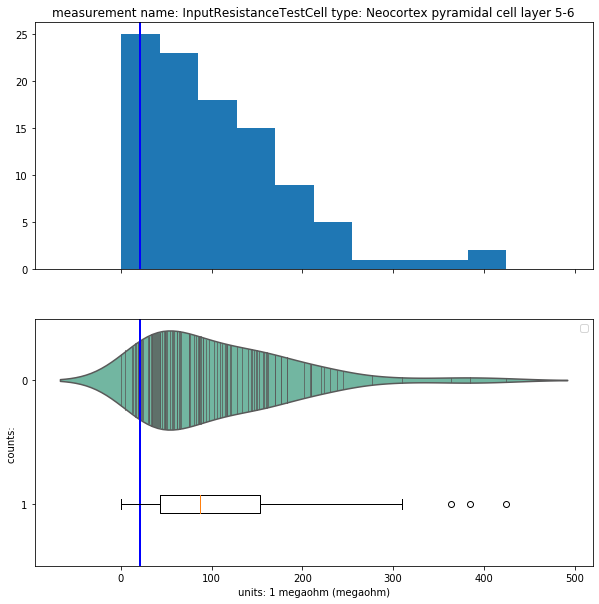
\includegraphics[width=0.7\linewidth]{notebooks_conver%ted/needata_thesis_files/needata_thesis_5_13}
%    \end{center}
    
    
%    \begin{center}
%    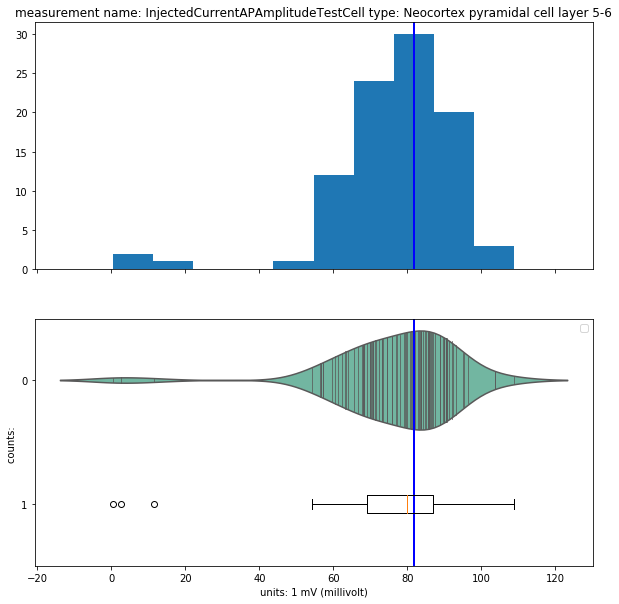
\includegraphics[width=0.7\linewidth]{notebooks_converted/needata_thesis_files/needata_thesis_5_16}
%    \end{center}

\begin{figure}
\begin{center}

     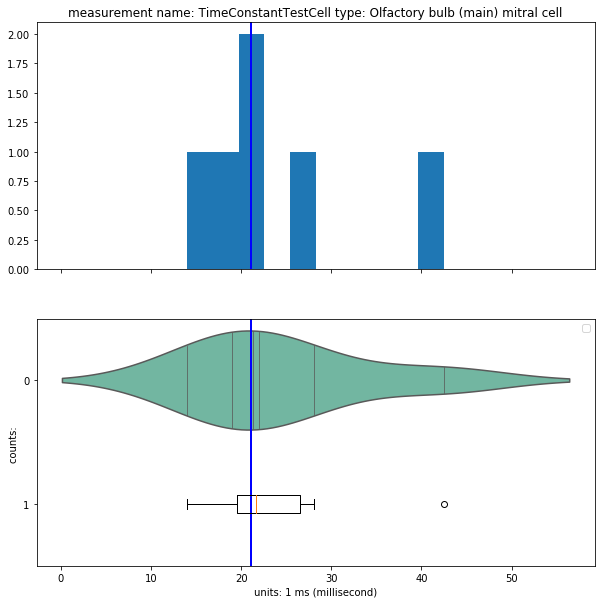
\includegraphics[scale=0.5]{notebooks_converted/needata_thesis_files/needata_thesis_5_23}
\caption{In the top panel of this plot we see a binned histogram of Neuro electro spike width measurements in the CA1 basket cell Neuron, in the bottom panel we see a violin plot, and a box plot of the same data. In both top and bottom panels, the mode is of the distribution is denoted by a blue vertical line. In this way the mode of the data distribution can be compared to the mean in the box plot. Often modes, and means of the measurements disagree, as they do in the case of CA1 basket cell spike widths. When consulting NeuroElectro measurement, a very common distribution shape is one which is possibly uniform, or multi-modal. It is perhaps obvious but worth noting that a uniform distribution, is not well described by a normal distribution. Under a normal distribution a range of measurement values are equally likely to occur.}
\end{center}

\end{figure}

   